\section{Reactive approach}
\label{exp:reactive}

This section presents performance results related to the evaluation of \rSPS{} and its ability to adapt to the dynamics of the data stream, without reducing the rate of processed events.

The evaluation is composed of two parts: (1) a comparison of \rSPS{} with different configurations (Section \ref{exp:ra-weight}); and (2) evaluation results of a tweet-based more complex application (Section \ref{exp:ra-complex}).


\subsection{Weight evaluation}
\label{exp:ra-weight}
The current experiment aims at evaluating the performance of \rSPS{}, which are based on the $\delta$ value (see Equation \ref{eq:rsps-delta}) and the weights (see Table \ref{tab:exp-reactive-parameters}). We used the \textit{Twitter Smoothed} dataset, \textit{Twitter linear - Detection} application, and \textit{Shuffle grouping} for stream grouping strategy. For calculating the \textit{Saved resources} metric, we have fixed $r_{over} = 40$ (i.e., $r_i = 10$). The size of each pool of replicas ($p$) was set to 50.

In order to quantify the impact of $U$ and $Q$ in the adaptation process, we evaluate them independently. The results of the 3 metrics are presented in Table \ref{tab:exp-ra-twitter-linear}.

\begin{table}[!ht]
\centering
\begin{tabular}{|l|llll|}
\hline
 & \begin{tabular}[c]{@{}l@{}}Saved\\ Nodes\end{tabular} & \begin{tabular}[c]{@{}l@{}}Throughput\\ Degradation\end{tabular} & \begin{tabular}[c]{@{}l@{}}Diff. Processed\\ Events\end{tabular} & \begin{tabular}[c]{@{}l@{}}Latency\\ (ms)\end{tabular} \\ \hline \hline
$\delta$ & 0.3996  & 0.1092 & 0.8907 & 39687.51 \\ \hline
U        & -0.8934 & 0.2597 & 0.7402 & 23441.39 \\ \hline
Q        & 0.4975  & 0.6830 & 0.3169 & 28799.60 \\ \hline
\end{tabular}
\caption{System metric values of  $\delta$, U, and Q using \textit{Twitter Smoothed} dataset.}
\label{tab:exp-ra-twitter-linear}
\end{table}

Figure \ref{fig:exp-ra-twitter-linear-replicas} shows the number of active replicas for each metric. A considerable increase in active replicas is observed in the first third of the three experiments. Then, in the second period, since the $U$ experiment only analyzes if another replica is necessary to improve operator utilization, it continues to increase the active replicas, which generates a decrease in the performance of the system, due to the overhead of managing a high number of replicas. Likewise, in Table \ref{tab:exp-ra-twitter-linear}, the \textit{Saved nodes} metric shows that the experiment with metric $U$ requires $129.3\%$ more active replicas than the one with $\delta$ metric. Note that for the $U$ metric, we observe a negative value of saved nodes since sometimes the number of replicas becomes greater than the overestimated value. On the other hand, the  $Q$ metric has a $24.5\%$ \textit{Saved nodes} improvement over the $\delta$ metric but it succeeds to process only less than $32\%$ of events whereas $\delta$ metric can process more than $89\%$ of events.

\begin{figure}[!ht]
    \centering
    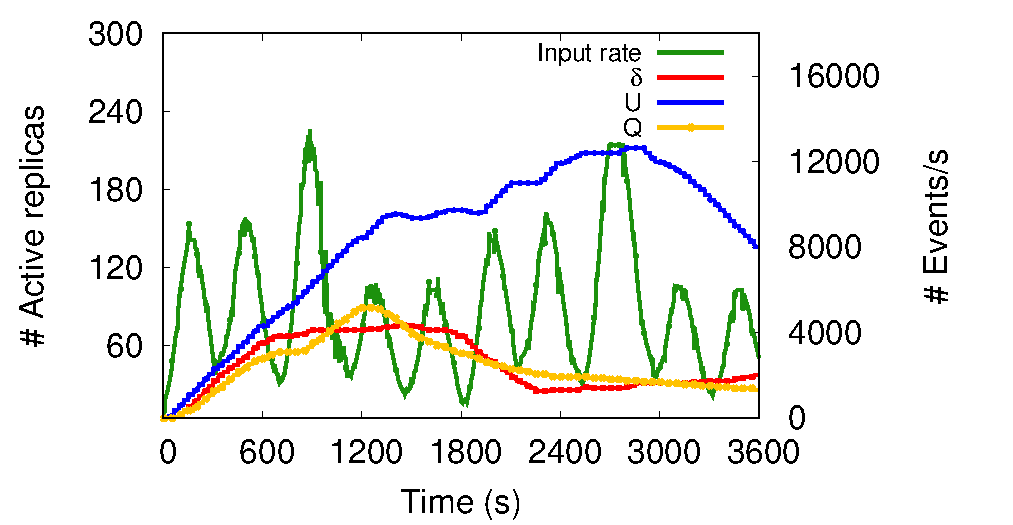
\includegraphics[width=0.75\textwidth]{figures/exp/reactive/TwitterLinear-Replicas.pdf}
    \caption{Total number of active replicas of $\delta$, U, and Q.}
    \label{fig:exp-ra-twitter-linear-replicas}
\end{figure}

The behaviour of $\delta$, $Q$, $U$ output rate as well as input rate are shown in Figure \ref{fig:exp-ra-twitter-linear-throughput}. Regarding the three metrics, they are similar in the first and second peaks but not in the third one, since the $Q$ experiment was not able to process events similarly to the other two: the queue increased, generating an overload in the system, which led the application to crash after the fourth peak. On the other hand, both the $ \delta $ and $U$ experiments continue to process events, until the eighth peak, which generates a saturation in the system of the $U$ experiment, making the application to crash after the ninth peak. As mentioned above, a large number of active replicas induces an overhead for handling them, decreasing the performance of the system. We also observe that there is a $15.05\%$ difference between the $ \delta $ and U regarding the \textit{Throughput degradation} metric (Table \ref{tab:exp-ra-twitter-linear}), which indicates a higher stability of  $ \delta $ experiment then $U$ one. Also, due to the early instability of the $Q$ experiment, there is a difference of $57.38\%$ with respect to the $ \delta $ one. 

\begin{figure}[!ht]
    \centering
    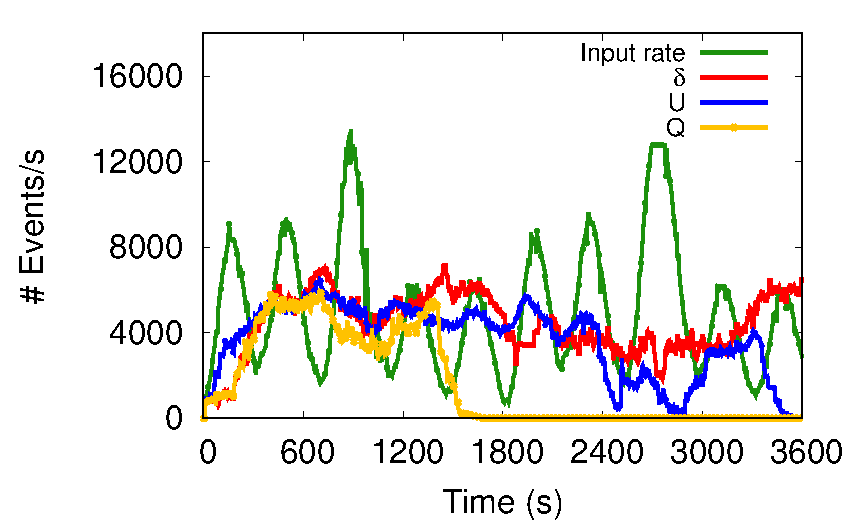
\includegraphics[width=0.75\textwidth]{figures/exp/reactive/TwitterLinear-Throughput.pdf}
    \caption{Throughput of  $\delta$, U, and Q.}
    \label{fig:exp-ra-twitter-linear-throughput}
\end{figure}

The total number of processed events is shown in Figure \ref{fig:exp-ra-twitter-linear-exec-total}. Because of application crash, after $ t = 1600s$ (resp., $ t = 3300s $) the curve is a constant for the $Q$ (resp., $U$) experiment. The difference using $\delta$ instance with respect to $U$ and $Q$ is $15.05\%$ and $57.3 \%$ respectively (Table \ref{tab:exp-ra-twitter-linear}).  

\begin{figure}[!ht]
    \centering
    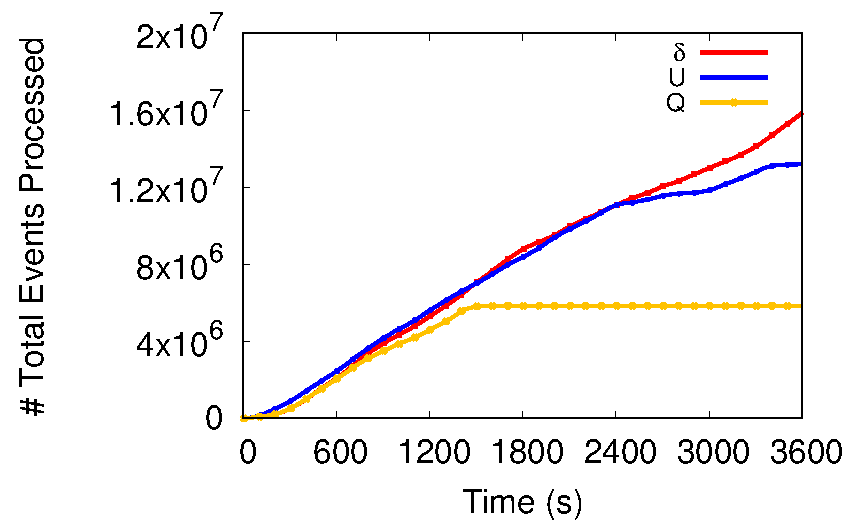
\includegraphics[width=0.75\textwidth]{figures/exp/reactive/TwitterLinear-ExecutedTotal.pdf}
    \caption{Total number of processed events of $\delta$, U,  and  Q.}
    \label{fig:exp-ra-twitter-linear-exec-total}
\end{figure}

Figure \ref{fig:exp-ra-twitter-linear-latency} presents the latency of the three metrics. At $ t = 1600s $, there is a strong rise in the latency for Q until the application crashes. The same happens at $ t = 3300s $ for the $U$ experiment. Due to the number of events and the system overload, the latest queued events can not been processed. The system becomes then saturated and is not able to continue processing. On the other hand, the latency with $ \delta $ is on average higher, but the system is capable of processing a greater number of events. Therefore, although the $ \delta $ instance does not have better performance in terms of latency, it is able of processing a greater amount of data without having to cope with the problem of over or under estimated  number of per operator replicas, as in the case of $U$ and $Q$ experiments respectively. The $ \delta $ latency increase  relative to $U$ and $Q$ is $69.3\%$ and $37.8\%$ respectively. 

\begin{figure}[!ht]
    \centering
    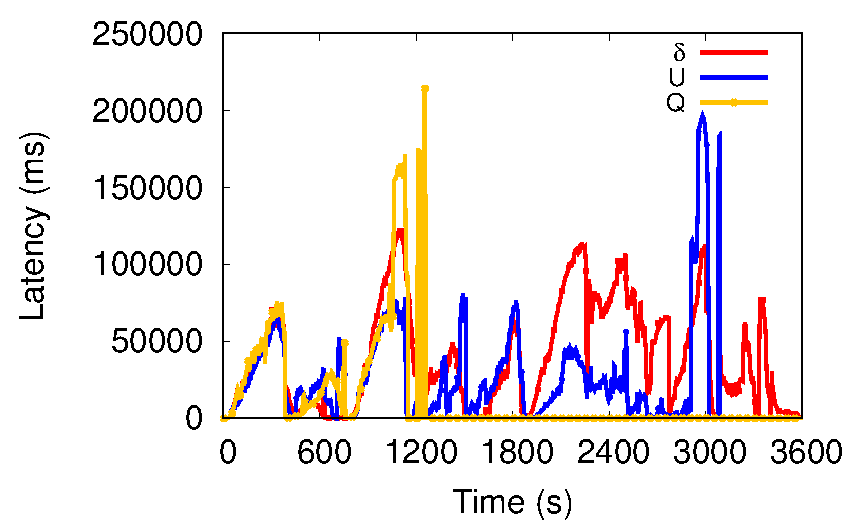
\includegraphics[width=0.75\textwidth]{figures/exp/reactive/TwitterLinear-Latency.pdf}
    \caption{Latency of $\delta$, U, and Q. }
    \label{fig:exp-ra-twitter-linear-latency}
\end{figure}


\subsection{Complex application}
\label{exp:ra-complex}
We have also evaluated \rSPS{} with a complex application. For this experiment, we have compared \rSPS{} with an overprovisioning Storm which always uses a fixed number of replicas per operator, denoted $S_{over}$. Such numbers are fixed ($r_i=5$) at the beginning of the data processing and do not vary during the experiment. We used the \textit{Twitter Smoothed} dataset, \textit{Twitter complex} application, and \textit{Shuffle grouping} for stream grouping strategy. For calculating the \textit{Saved resources} metric, we have fixed $r_{over} = 40$ (i.e., $r_i = 5$). The size of each pool of replicas ($p$) was set to 6.

Table \ref{tab:exp-ra-twitter-complex} presents the results of both systems, \rSPS{} and $S_{over}$. Due to the time gap to process events, we observe a $42.52\%$ difference between \textit{Throughput degradation} values of the two systems. However, such a difference is not a real problem since the numbers of processed events of the two systems are quite close, as shown in the same table.
On the other hand, in \rSPS{}, we observe a high reduction of used resources with $50.23\%$ fewer active replicas, when compared to $S_{over}$.
Also, in this application, \rSPS{} succeeded to process almost $98\%$ of the total events while consuming  $2.7$ times less CPU than the static configuration which overestimates the number of replicas.

\begin{table}[!ht]
\centering
\begin{tabular}{|c|llll|}
\hline
System & \begin{tabular}[c]{@{}l@{}}Saved\\ Nodes\end{tabular} & \begin{tabular}[c]{@{}l@{}}Throughput\\ Degradation\end{tabular} & \begin{tabular}[c]{@{}l@{}}Diff. Processed\\ Events\end{tabular} & \begin{tabular}[c]{@{}l@{}}Latency\\ (ms)\end{tabular} \\ \hline \hline
$\delta$ & 0.5023 & 0.4252 & 0.98 & 179.5401 \\ \hline
$S_{over}$ & 0 & 0 & 1.00 & 31.990\\ \hline
\end{tabular}
\caption{System metric values of \rSPS{} and $S_{over}$ using \textit{Twitter Smoothed} dataset and Twitter complex application.}

\label{tab:exp-ra-twitter-complex}
\end{table}

\subsection{Discussion}
We have evaluated \rSPS{} based on $\delta$ metric which aggregate three metrics, the average load of the operator ($U$), the average execution time of an event ($E$), and the operator input queue ($Q$) for characterizing the state of an operator at runtime. By assigning a weight to each of these metrics, \rSPS{} can decide whether the operator is overloaded, underloaded or stable, respectively increasing, reducing, or keeping the same number of active replicas. Performance results with Twitter input data and different evaluation metrics confirm the advantages of using the three metrics compared to a single one. %Thus, we have also evaluated a solution that has great potential, because it does not only analyse one metric, but different factors of the SPS, either physical or logical, which can help to improve its performance.
